\chapter{Main Body}
\label{cha:Main Body}

\section{Trigger R\&D}
\label{sec:Trigger}
To trigger the counter of the WSB, there are a few possible solutions. The remote has to be wearable, and it has to be triggered during the game. This is hard to implement, because a usual button is too tiny to press during a game, and it can be frustrating to always aim for the trigger button. Therefore, I decided to use an accelerometer and count the points by simply tapping on the thigh. My idea is to mount the WSB remote on the inside of the thigh or as a knee pad replacement for example in volleyball. Then the vibrations/accelerations travel through the user's body and get measured by the WSB remote. But this can be rather hard, because during sports the body is always accelerating, and it could be hard to distinguish from a usual movement or a "thigh tip". If the accelerometer idea doesn't work out, I would use flexible membrane buttons to control the WSB. 

\subsection{Accelerometer R\&D}
\label{ssec:Accelerometer}
At my current lab at ETH I found an accelerometer to test out, if I can use it as a trigger.
\subsubsection{control LSM303C accelerometer}
Attention: Mind that the CS\_XL and CS\_MAG have to be pulled up to enable I\textsuperscript{2}C mode. and use external I\textsuperscript{2}C pullups, because on MKI163V1 devBoard are no pullup R's.

slave address: 0b00111010 = 0x3A \cite{DS_LSM303C}

\begin{figure}[H]
	\centering
	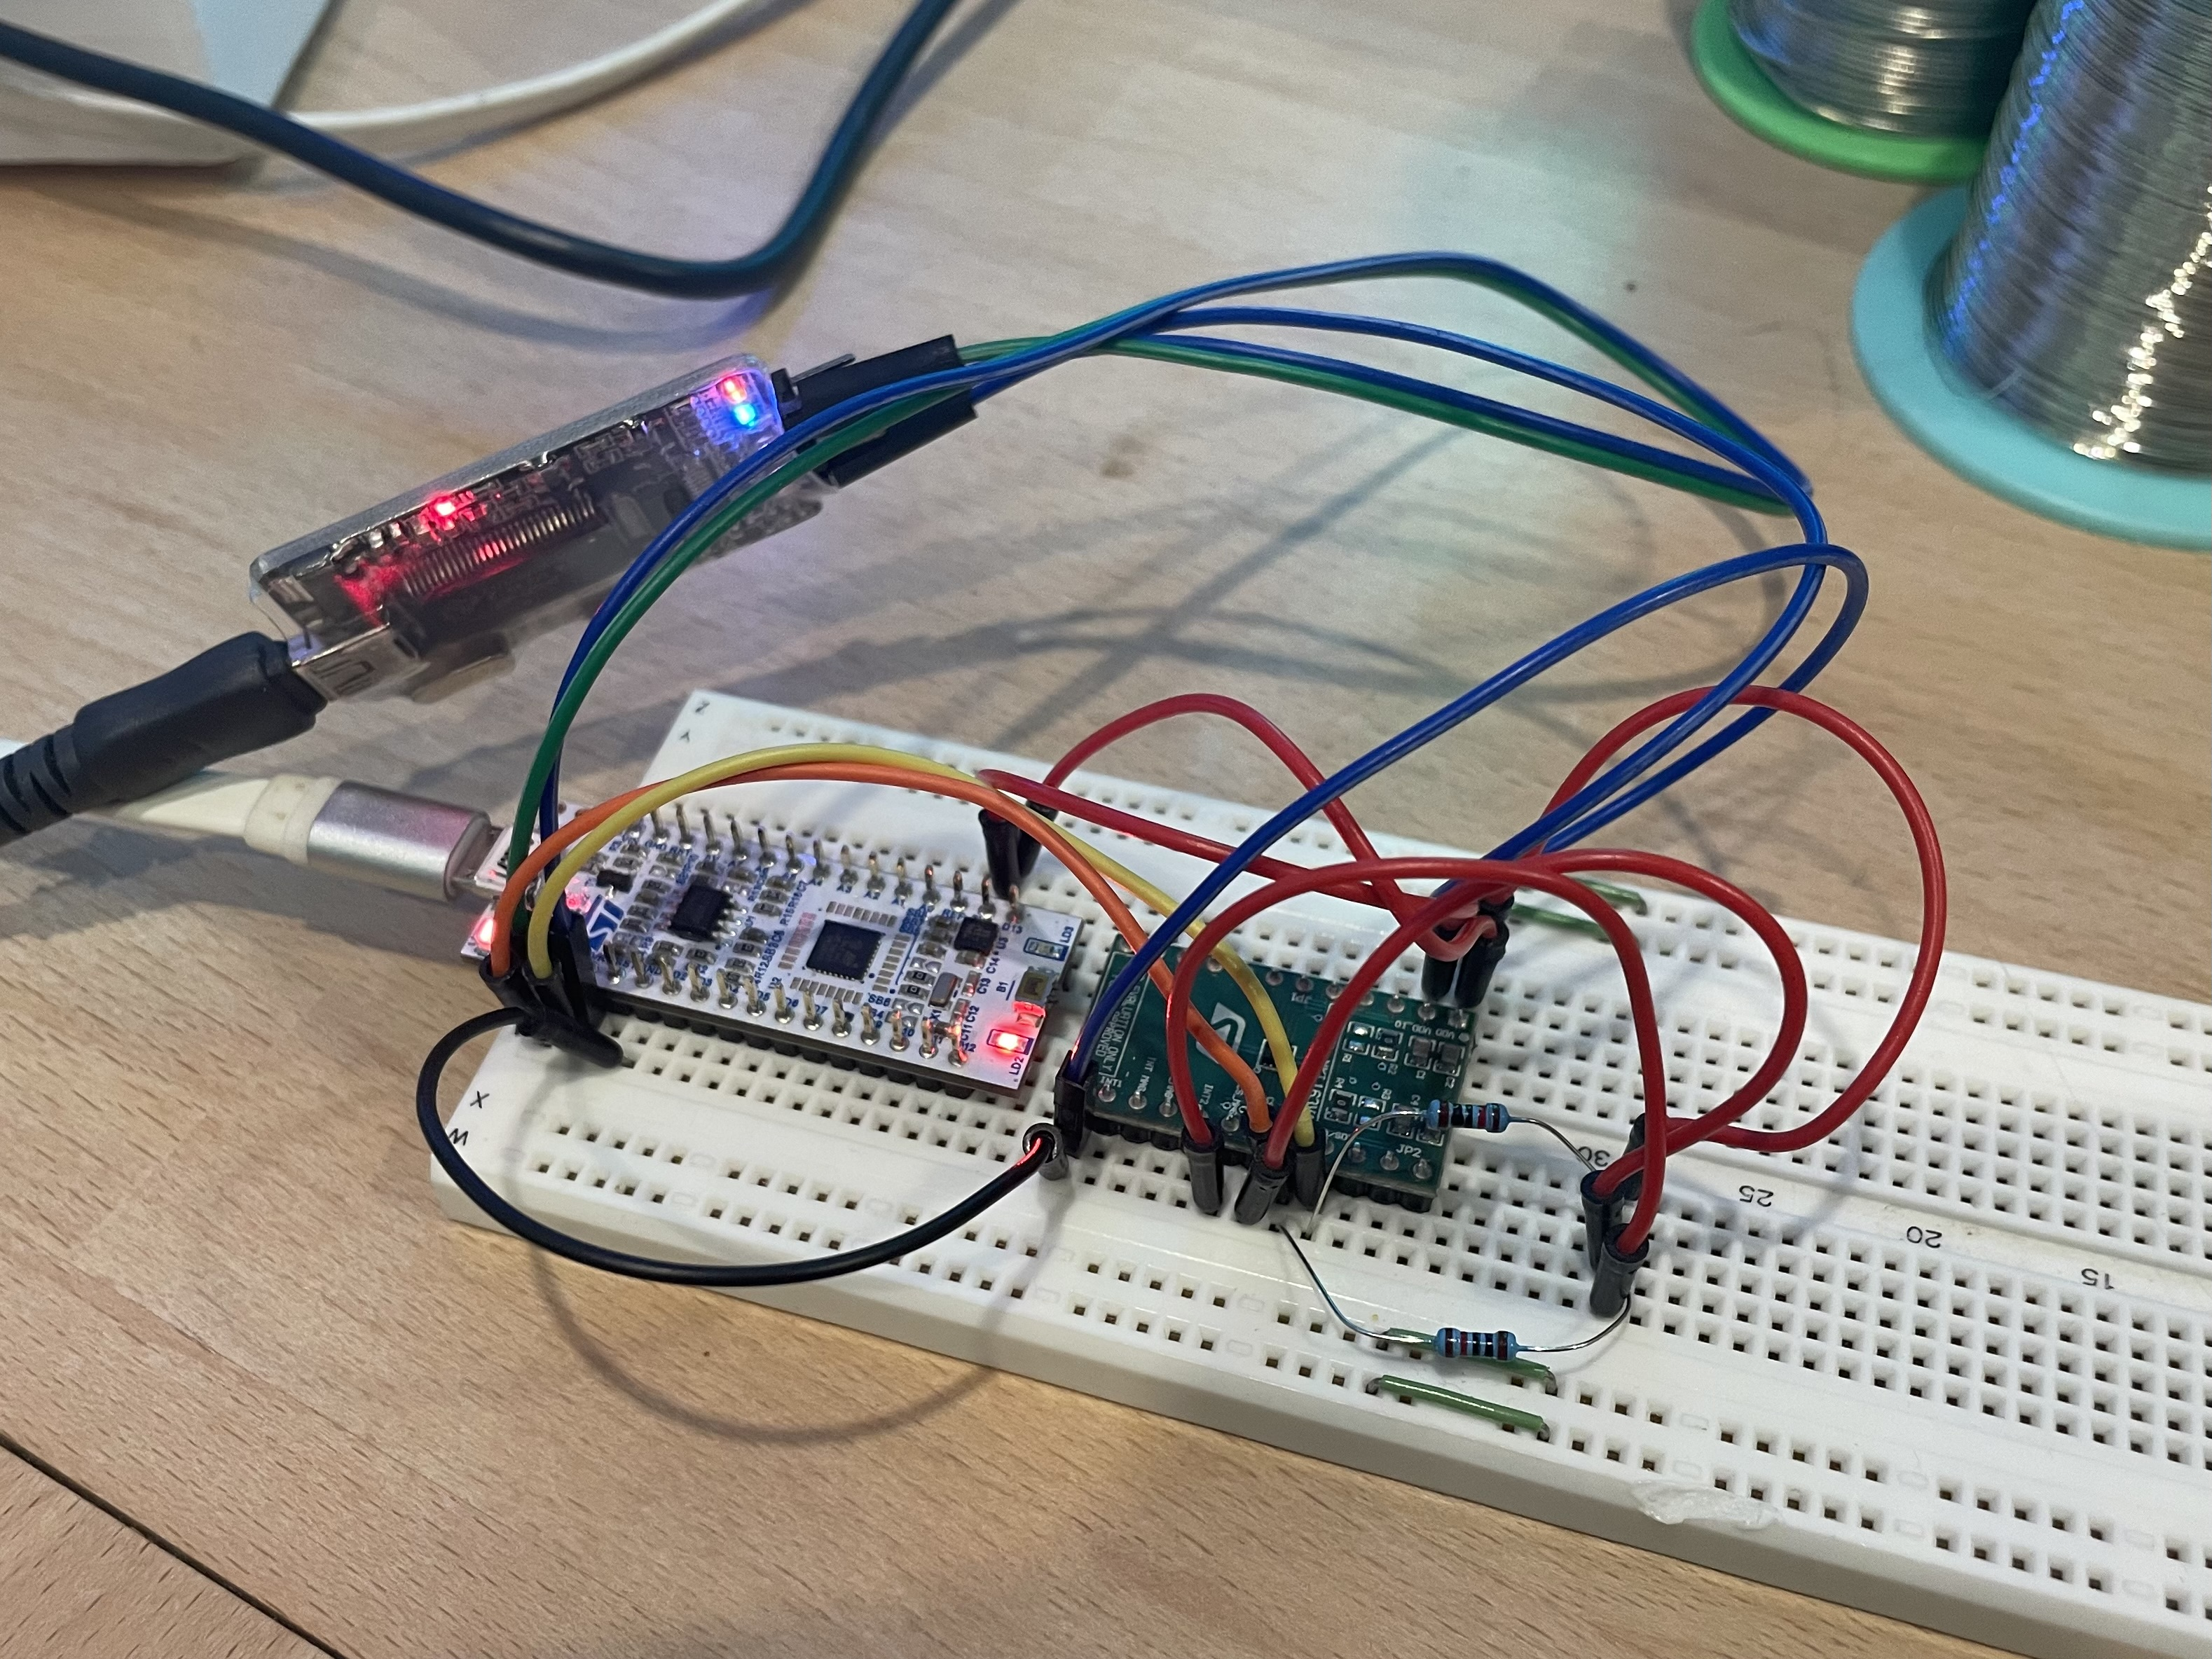
\includegraphics[width=10cm]{Resources/accTestLab.jpeg}
	\caption{Accelerometer test: setup}
	\label{fig:accTestLab}
\end{figure}

\subsubsection{First test the "WHO AM I" register}
Communication test: reg 0x0F should read as 0x41

\subsubsection{Read acceleration}
CTRL\_REG1\_A (0x20): 0x3F (Enable XYZ, 100Hz, block data overwriting)

CTRL\_REG2\_A (0x21): 0x00 (disable LPF)

CTRL\_REG3\_A (0x22): 0x00 (disable interrupts)

CTRL\_REG4\_A (0x23): 0x34 (enable I\textsuperscript{2}C, enable auto address increments, FS $\pm$8g)

CTRL\_REG5\_A (0x24): 0x00

CTRL\_REG6\_A (0x25): 0x00

CTRL\_REG7\_A (0x26): 0x00
\\

STATUS\_REG\_A (0x27):
Bit 3 set if xyz data is available / Bit 8 set if xyz data overrun.

OUT\_X\_L (0x28)(2bytes)   (0.061mg/LSB) @ FS=8g

OUT\_Y\_L (0x2A)(2bytes)   (0.061mg/LSB) @ FS=8g

OUT\_Z\_L (0x2C)(2bytes)   (0.061mg/LSB) @ FS=8g

\begin{figure}[H]
	\centering
	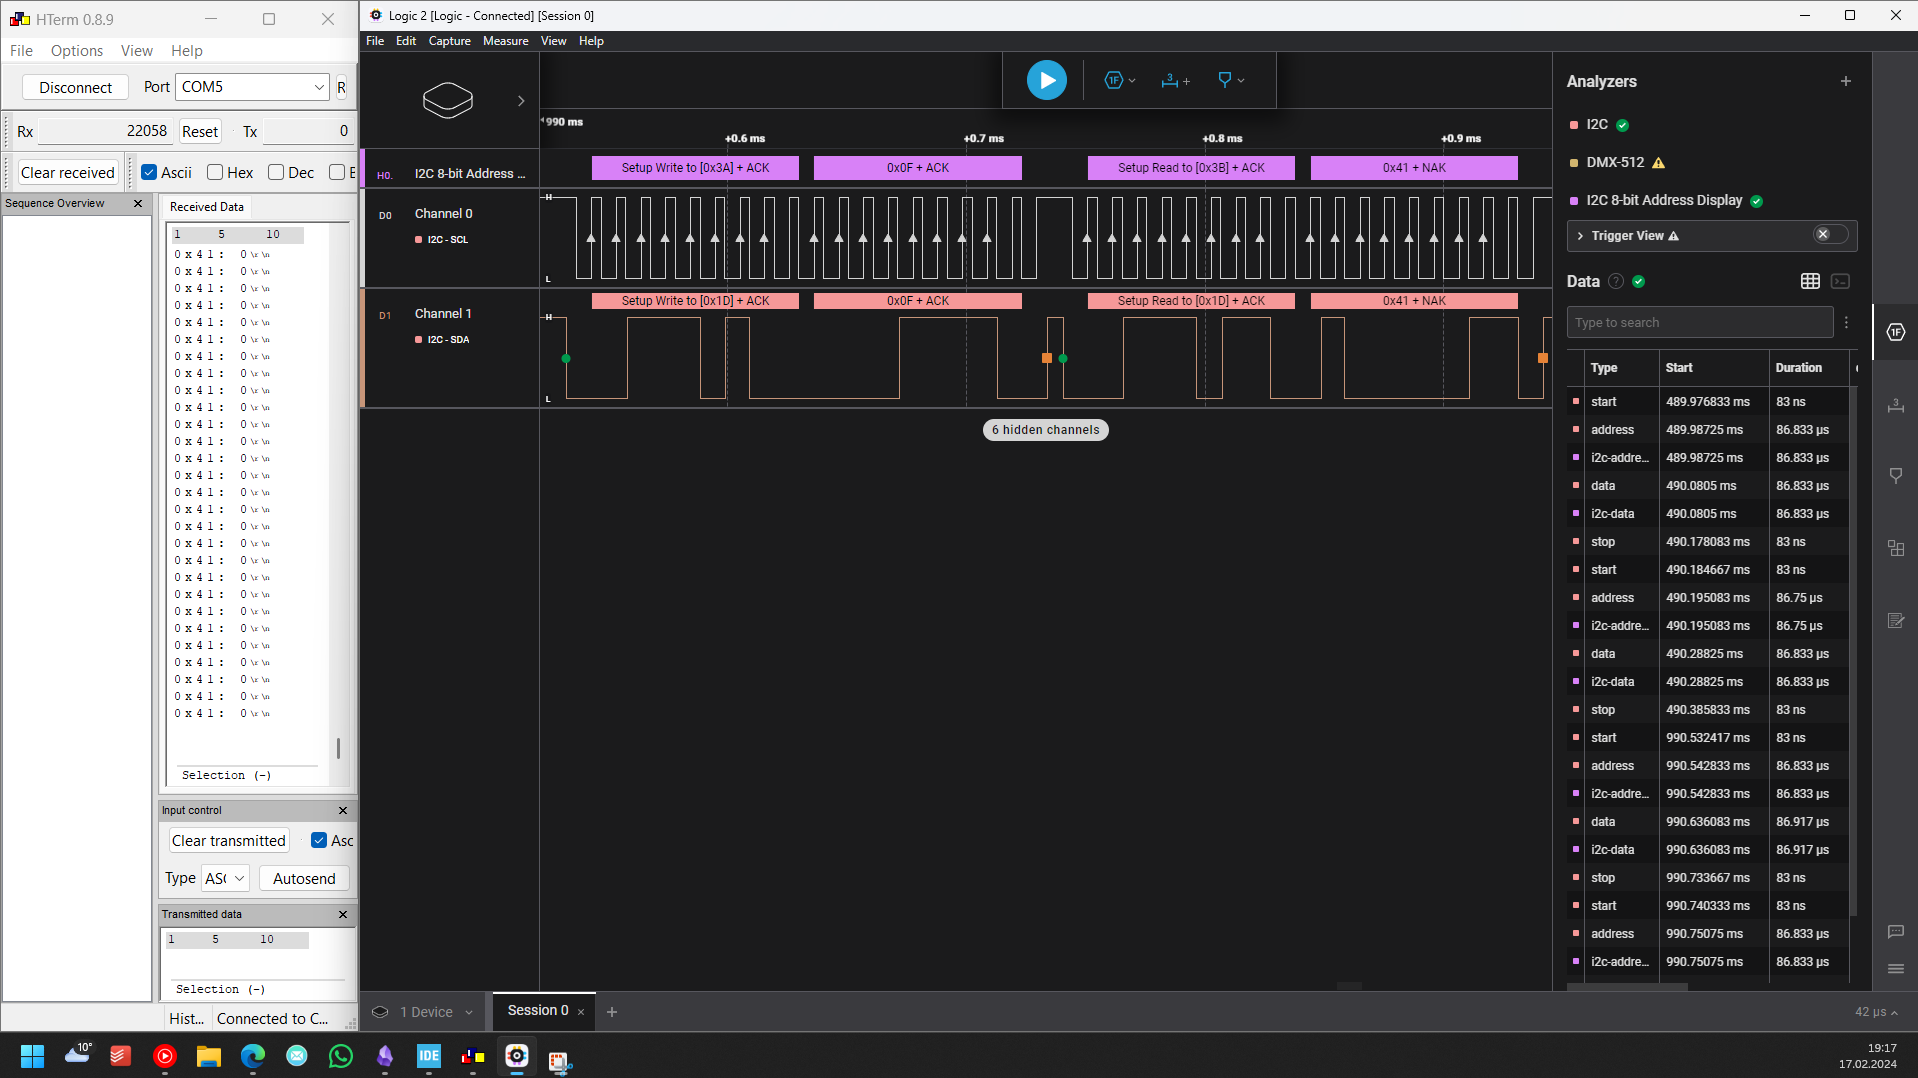
\includegraphics[width=17cm]{Resources/accTestLA.png}
	\caption{Accelerometer test: logic analyzer}
	\label{fig:accTestLA}
\end{figure}
\newpage

\subsubsection{Test Results}
After looking at the measurement results, I decided that it would be best to populate an accelerometer and the membrane buttons on the PCB, that I have an alternative if the accelerometer doesn't work out. Because it's hard to analyze if the accelerometer as trigger will work out during a game and I can't attach the current breadboard to my thigh to test the accelerometer out. But for the final design I'll probably choose the "STM LIS2HH12" accelerometer.

\begin{figure}[H]
	\centering
	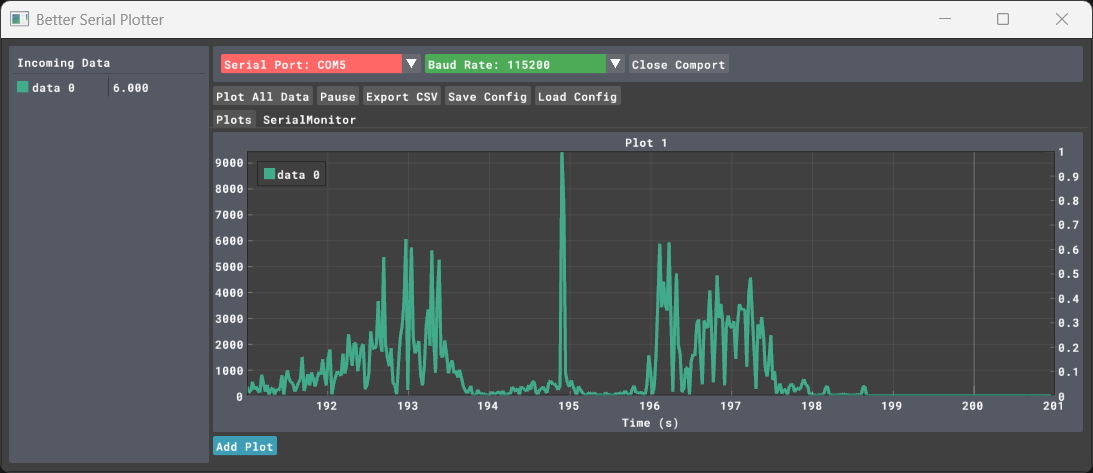
\includegraphics[width=17cm]{Resources/accTestMeas.png}
	\caption{Accelerometer test: results}
	\label{fig:accTestMeas}
\end{figure}

I hope that I can differentiate normal sports movement from "thigh taps" by looking at the momental acceleration. In Fig: \ref{fig:accTestMeas}, the middle pulse was a "thigh tap" and the first and last ones are movement from the body, which take a lot longer but don't peak out as high. The shown data is actually the variable "accDelta" from the "6\_Software/dev/LSM303C\_Test/Core/Src/ main.c" file.

\section{Battery Charging R\&D}
\label{sec:Battery Charging}
I'm sure, that I'll have to somehow power the WSB Remote as well as the WSB. Because they both have to be portable, I'm planning to use a rechargeable battery. For example Lithium Ion battery. And to use this battery I'll have to implement some protection circuits, as well as charging circuits. Important protection features are:
\begin{itemize}
    \item UVP - Under Voltage Protection (So the battery doesn't get broken)
    \item OVP - Over Voltage Protection (So the battery doesn't get broken)
    \item OTP - Over Temperature Protection (So the battery doesn't overheat or starts burning)
    \item OCP - Over Current Protection (So the circuits don't break)
\end{itemize}

So I started searching for LiIon charging ICs and I had looks at TIs ICs, like the "BQ25180YBGR" or "BQ25155YFPR". But the TI charging ICs are rather complicated and would take me too long to implement. Additionally after buying some samples of these ICs I recognized, that they are CSPs and really tiny, which makes them really hard to solder or make modifications on the PCB. So I got to my favourite semiconductor manufacturer STM and found the perfect IC, the STNS01. I also recognized, that STMs product portfolio is a lot smaller than TIs, which was quite overwhelming. STM only had about 5 ICs to choose from.


\section{Remote PCB}
\label{sec:Remote PCB}
The remote PCB connects all components together, such as the accelerometer, microcontroller and RF module. I decided to design a custom PCB and later order it, because there are too much and too small components to solder onto a development board. The WSBR PCB should have the following features according to the HW Concept. [\ref{sec:HW Concept}]

\begin{itemize}
    \item Battery charging through USB-C with battery level monitoring.
    \item Battery level monitoring when power button is pressed once.
    \item Start remote, when power button is pressed once and then again for longer.
    \item Flash MCU using USB-DFU mode when pressing the boot button.
    \item Use an accelerometer or three membrane buttons as a trigger to count points.
    \item Send data via RF (nRF24L01) to WSB and show the remote state with an RGB LED.
\end{itemize}


\subsection{Schematics}
The schematics were drawn using Altium Designer and are stored in the "5\_Hardware\\WSBR\_Board" directory. Full Schematics here: [\ref{fig:Remote Schematics}]

\label{ssec:Schematics}

\subsubsection{Battery Management Circuit}
J1 (USB-C port) is used as the charging port. It is configured to deliver a maximum current of 3A according to Microchip AN1953 \cite{AN1953}. Additionally, the 2 data lines of J1 are tied to the microcontroller through an ESD protection IC (U2) to program it in the field without having to use an STLINK. For the commissioning, TP3 and TP4 are populated to power the PCB with a lab bench power supply.

The battery is charged to 4.2V through U4 (STNS01) using the CC-CV method. The fast charging current of U4 is set to 125mA using R5 \cite{DS_STNS01}. As long as the temperature stays between 0°C and 45°C, which is measured by R8 (shall be placed near to the battery).
$$I_{CHG}=\frac{U_{Iset} \cdot K}{R_5}=\frac{1V \cdot 200}{1.6k\Omega}=125mA$$

All components on the PCB are supplied by the LDO of U4, which has a constant output voltage of 3.1V. The main 3.1V rail is only enabled if U5 is turned on. This ensures that the battery isn't drained when the remote isn't even being used. The Load switches U5 \& U6 are enabled if at least one of the following conditions is met.
\begin{itemize}
    \item Power Button S3 is pressed. (Once pressed the MCU pulls the enable signal high.)
    \item The MCU pulls the enable signal high.
    \item USB-C connected, and therefore the battery is charging.
\end{itemize}
If the circuit for U5 doesn't work, there's an alternative switch (S4), to bridge the load switch and use as the new "but boring" power switch.

To measure the battery voltage and display the level, the MCU measures half of the battery voltage using its internal ADC and an external voltage divider (R10 \& R11).

\begin{figure}[H]
	\centering
        \framebox{
	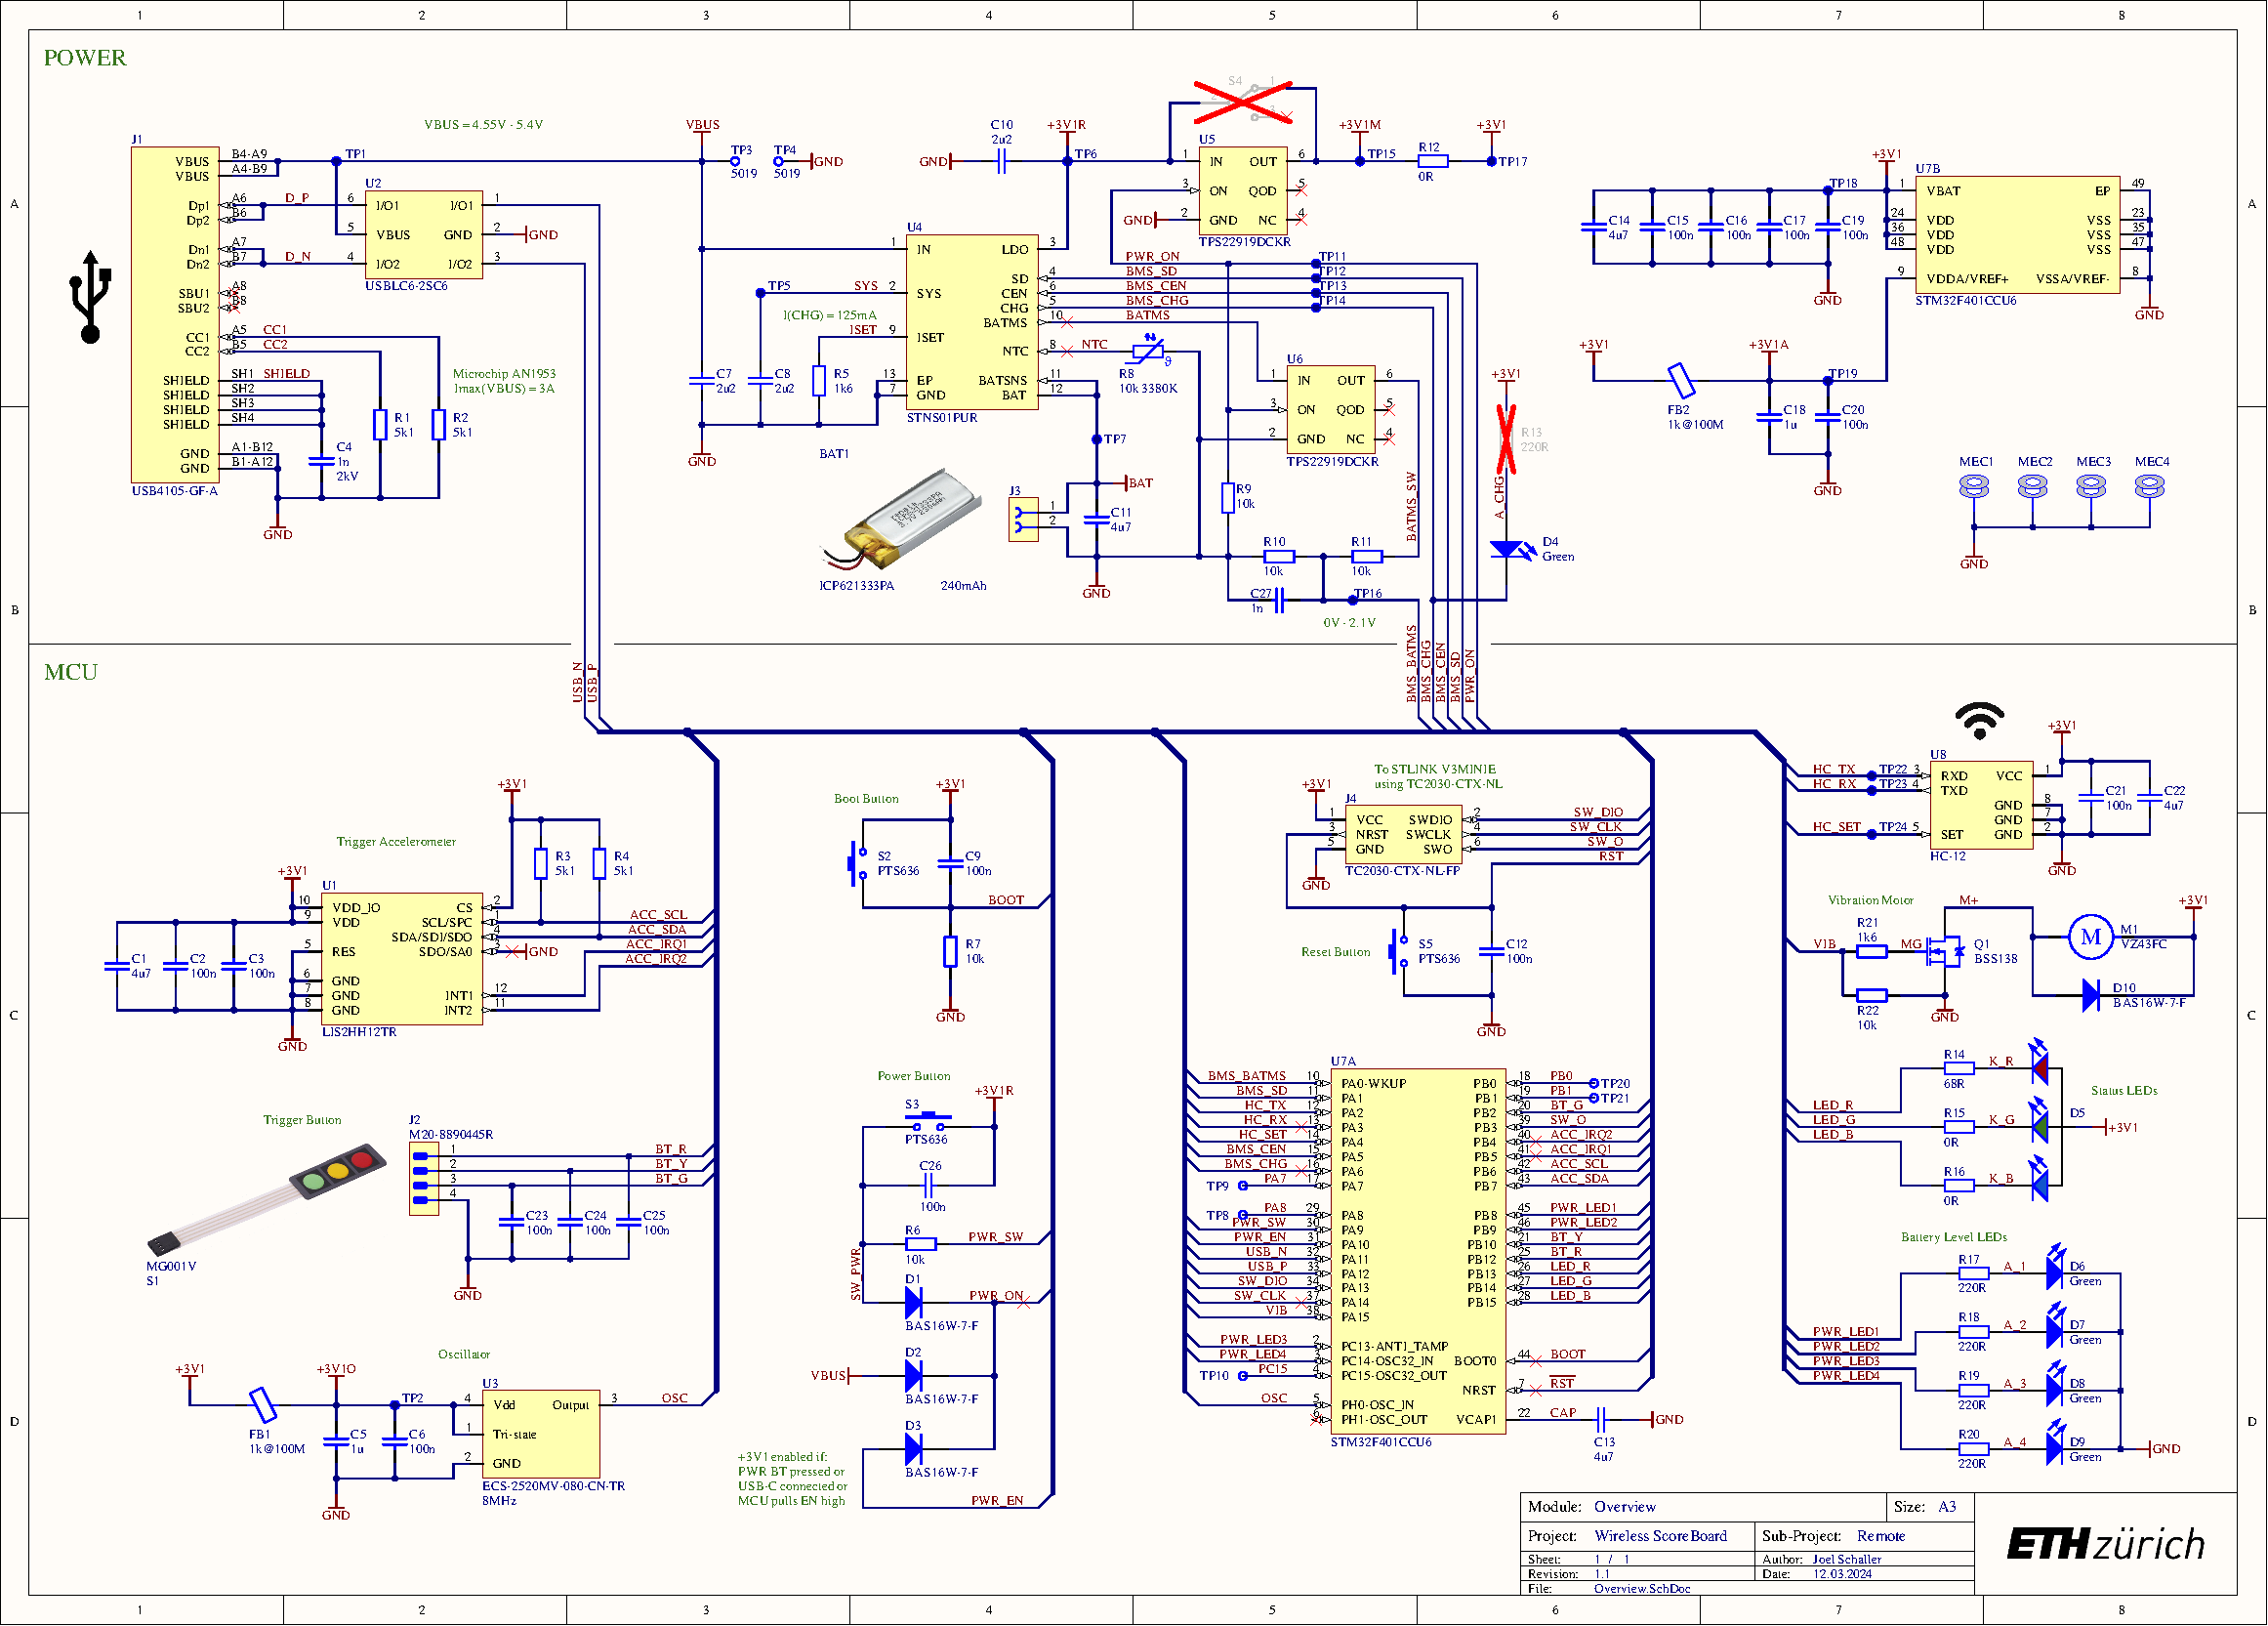
\includegraphics[width=16.7cm, trim={0.7cm 16cm 12cm 0.6cm}, clip, page=1]{../../5_Hardware/WSBR_Board/Project Outputs for WSBR_Board/WSBR_Board.PDF}}
	\caption{Battery Management Circuit}
	\label{fig:Battery Management Circuit}
\end{figure}